\documentclass{scrartcl}

\usepackage{tabularx} %better tables
\usepackage[table]{xcolor}
\usepackage[utf8]{inputenc}
\usepackage[ngerman]{babel}
\usepackage{hyperref}
\usepackage{tikz}
\usepackage{graphicx}

\begin{document}
	\section*{Einführungsbericht}
	
	\begin{tabularx}{\textwidth}{| X | X |}
	\hline
	Status & In Arbeit\\
	\hline
	Projektname & DARWIN\\
	\hline
	Projektleiter & Noe Thalheim\\
	\hline
	Auftraggeber & Stefan Schenk\\
	\hline
	Autoren & Yannik Dällenbach, Noe Thalheim\\
	\hline
	\end{tabularx}
	
	\subsection*{Änderungskontrolle}
	\begin{tabularx}{\textwidth}{| X | X | X |}
	\hline
	\rowcolor[gray]{0.9} Version & Datum & Beschreibung\\
	\hline
	1.0 & 12.05.2013 & Init\\
	\hline
	\end{tabularx}
	
	\pagebreak
	%inhaltsverzeichnis
	\tableofcontents
	\pagebreak
	%abschnitt 1
    \section{Zweck des Dokuments}
Zusammenfassung der Ergebnisse der Phase „Einführung“.

    \section{Einführungsplan}
\subsection{Vorgehen}
\subsection{Risiken}
\subsection{Grober Zeitplan für die Einführung}

    \section{Mittelbedarf}
%TODO Zusammenfassung

    \usetikzlibrary{arrows,positioning}
	
\section{Planung und Organisation}
	
\subsection{Projektorganisation}
An dem Projekt werden folgende Personen mitarbeiten:
\\\\
\begin{tikzpicture}[node distance=1cm, auto]  
\tikzset{
	    mynode/.style={rectangle,align=left,draw=black, top color=white, bottom color=white!50,very thick, inner sep=1em, minimum size=3em, text centered},
	    myarrow/.style={->, >=latex', shorten >=1pt, thick},
	    mylabel/.style={text width=7em, text centered} 
	}  
	\node[mynode] (auftraggeber) {\textbf{Auftraggeber}\\Stefan Schenk};  
	\node[mynode, below=1cm of auftraggeber] (projektleiter) {\textbf{Projektleiter}\\Noe Thalheim};  
	\node[mynode, right=of projektleiter] (projektmitarbeiter1) {\textbf{Projektmitarbeiter}\\Yannik Dällenbach};


	\draw[myarrow] [<->] (auftraggeber.south) -- (projektleiter.north);	
	\draw[myarrow] [-] (projektleiter.east) -- (projektmitarbeiter1.west);

	\end{tikzpicture} 
	\medskip

	Die Aufgabenverteilung wird das ganze Projekt gleich bleiben.
	
	\subsection{Termine}
	
	Für unser Projekt sind folgende Termine von Wichtigkeit:
	\begin{description}
		\item[] Starttermin: 05.02.2013
		\item[] Endtermin: 04.06.2013
	\end{description}
	Daraus ergibt sich für unser Projekt folgender Terminplan:
	\\ \\
	\tiny{
	\begin{tabular}{| p{2cm} | p{1cm} | p{1cm} | p{1cm} | p{1cm} | p{1cm} | p{1cm} |}
	\hline
	\rowcolor[gray]{0.9}  & 12.02.13 - 19.02.13 & 19.02.13 - 05.03.13 & 5.03.13 - 19.03.13 & 19.03.13 - 07.05.13 & 7.05.13 - 21.05.13 & 21.05.13 - 04.06.13 \\
	\hline
	Initialisierung & \cellcolor{yellow} & & & & & \\
	\hline
	Voranalyse & &  \cellcolor{yellow}& & & & \\
	\hline
	Konzept & & &  \cellcolor{yellow}& & & \\
	\hline
	Realisierung & & & &  \cellcolor{yellow}& & \\
	\hline
	Einführung & & & & & \cellcolor{yellow}& \\
	\hline
	Abschluss & & & & &  &\cellcolor{yellow} \\
	\hline
	\end{tabular}	
	}
	\small{
	\\ \\
	Unser Aufgabenplanung werden wir folgendermassen gestalten: 

	\begin{figure}[htb]

	\centering

	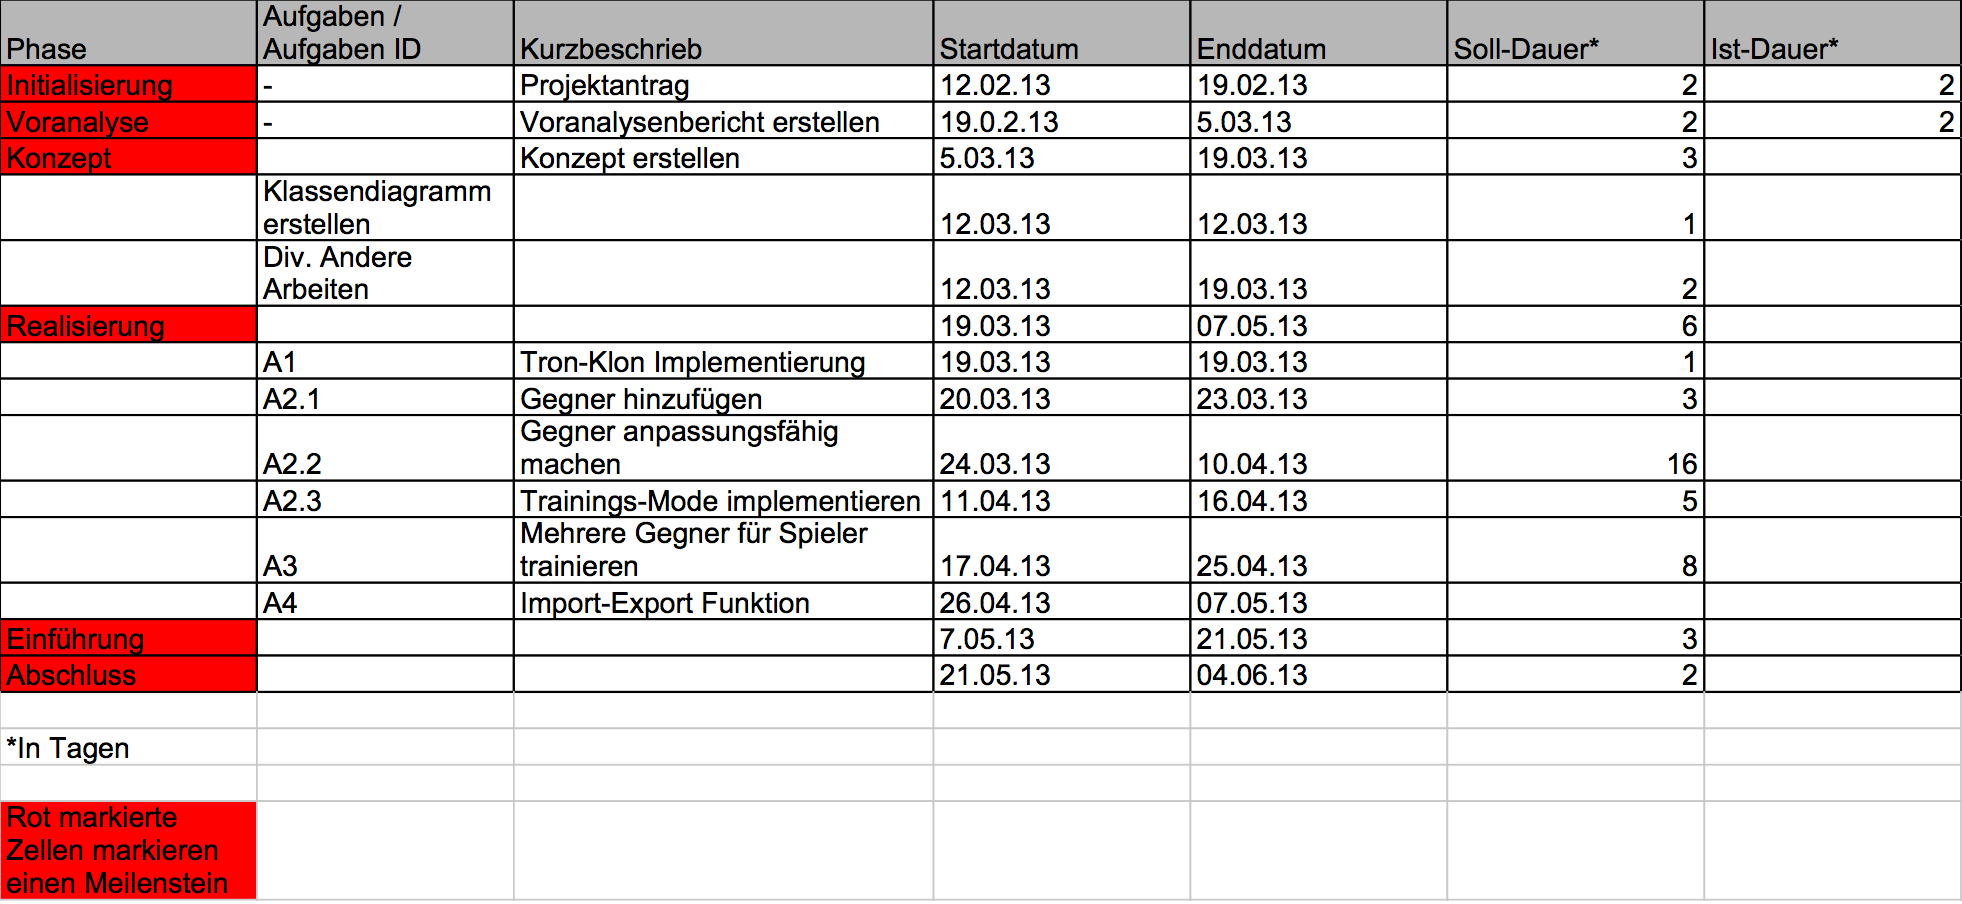
\includegraphics[width=\textwidth]{plan.png}

	\caption{Momentane Aufgabenplanung}

	\end{figure}

	\subsection{Prioritäten}
	Unsere Prioritäten für dieses Projekt sind das Verstehen und Implementieren von Evolutionären Algorithmen und somit das Selbststudium in diesen Gebieten. Zudem ist es uns wichtig durch dieses Projekt Erfahrungen im Zusammenhang mit der Programmierung in Objective-C sammeln zu können. 
}
    \section{Wirtschaftlichkeit}
%TODO import

    \section{Konsequenzen}
%TODO import

    \section{Antrag auf Freigabe der nächsten Projektphase}
Ich beantrage die Genehmigung des vorliegenden Konzeptberichts und die Freigabe für die Phase Realisierung durch den Auftraggeber, sowie die Kenntnisnahme des Projektfortschrittes durch den Studienbegleiter.

\\ \\ \\
Noe Thaleim:
\\ \\
\parbox{4cm}{\hrule
\strut \centering\footnotesize Ort, Datum} \hfill\parbox{4cm}{\hrule
\strut \centering\footnotesize Unterschrift}
\\ \\ \\
Yannik Dällenbach:
\\ \\
\parbox{4cm}{\hrule
\strut \centering\footnotesize Ort, Datum} \hfill\parbox{4cm}{\hrule
\strut \centering\footnotesize Unterschrift}
\\ \\ \\
Für den Auftraggeber:
\\ \\
\parbox{4cm}{\hrule
\strut \centering\footnotesize Ort, Datum} \hfill\parbox{4cm}{\hrule
\strut \centering\footnotesize Unterschrift}


\end{document}
